% !TEX root = paper-graphnet.tex

\section{Introduction}
\label{sec:intro}

Low-dimensional  vector embeddings of nodes in large graphs\footnote{While it is common to refer to these data structures as social or biological \emph{networks}, we use the term \emph{graph} to avoid ambiguity with neural network terminology.} have proved extremely useful as feature inputs for a wide variety of prediction and graph analysis tasks \cite{cao2015grarep,grover2016node2vec,perozzi2014deepwalk,tang2015line,wang2016structural}.
The basic idea behind node embedding approaches is to use dimensionality reduction techniques to distill the high-dimensional information about a node's graph neighborhood into a dense vector embedding. 
These node embeddings can then be fed to downstream machine learning systems and aid in tasks such as node classification, clustering, and link prediction \cite{grover2016node2vec,perozzi2014deepwalk,tang2015line}.

However, previous works have focused on embedding nodes from a single fixed graph, and many real-world applications require embeddings to be quickly generated for unseen nodes, or entirely new (sub)graphs. 
This inductive capability is essential for high-throughput, production machine learning systems, which operate on evolving graphs and constantly encounter unseen nodes (e.g., posts on Reddit, users and videos on Youtube).
An inductive approach to generating node embeddings also facilitates generalization across graphs with the same form of features:
for example, one could train an embedding generator on protein-protein interaction graphs derived from a model organism, and then easily produce node embeddings for data collected on new organisms using the trained model. 

The inductive node embedding problem is especially difficult, compared to the transductive setting, because generalizing to unseen nodes  requires ``aligning'' newly observed subgraphs to the node embeddings that the algorithm has already optimized on. 
An inductive framework must learn to recognize structural properties of a node's neighborhood that reveal both the node's local role in the graph, as well as its global position. 
 
 Most existing approaches to generating node embeddings are inherently transductive.
 The majority of these approaches directly optimize the embeddings for each node using matrix-factorization-based objectives, and do not naturally generalize to unseen data, since they make predictions on nodes in a single, fixed graph \cite{cao2015grarep,grover2016node2vec,ng2001spectral,perozzi2014deepwalk,tang2015line,
 wang2016structural,wang2017community,xu2017embedding}.
 These approaches can be modified to operate in an inductive setting (e.g., \cite{perozzi2014deepwalk}), but these modifications tend to be computationally expensive, requiring additional rounds of gradient descent before new predictions can be made. 
 There are also recent approaches to learning over graph structures using convolution operators that offer promise as an embedding methodology \cite{kipf2016semi}.
 So far, graph convolutional networks (GCNs)  have only been applied in the transductive setting with fixed graphs \cite{kipf2016semi,kipf2016variational}. 
 In this work we both extend GCNs to the task of inductive unsupervised learning and propose a framework that generalizes the GCN approach to use trainable aggregation functions (beyond simple convolutions). 

\xhdr{Present work} We propose a general framework, called \name\ (\textsc{sa}mple and aggre\textsc{g}at\textsc{e}), for inductive node embedding.
Unlike embedding approaches that are based on matrix factorization, we leverage node features (e.g., text attributes, node profile information, node degrees) in order to learn an embedding function that generalizes to unseen nodes. 
By incorporating node features in the learning algorithm, we simultaneously learn the topological structure of each node's neighborhood as well as the distribution of node features in the neighborhood.
While we focus on feature-rich graphs (e.g., citation data with text attributes, biological data with functional/molecular markers), our approach can also make use of structural features that are present in all graphs (e.g., node degrees).
Thus, our algorithm can also be applied to graphs without node features.

Instead of training a distinct embedding vector for each node, we train a set of {\em aggregator functions} that learn to aggregate feature information from a node's local neighborhood (Figure \ref{fig:overview}).
Each aggregator function aggregates information from a different number of hops, or search depth, away from a given node. 
At test, or inference time, we use our trained system to generate embeddings for entirely unseen nodes by applying the learned aggregation functions. 
Following previous work on generating node embeddings, we design an unsupervised loss function that allows \name\ to be trained without task-specific supervision.
We also show that \name\ can be trained in a fully supervised manner. 

\begin{figure}
\vspace{-20pt}
\centering
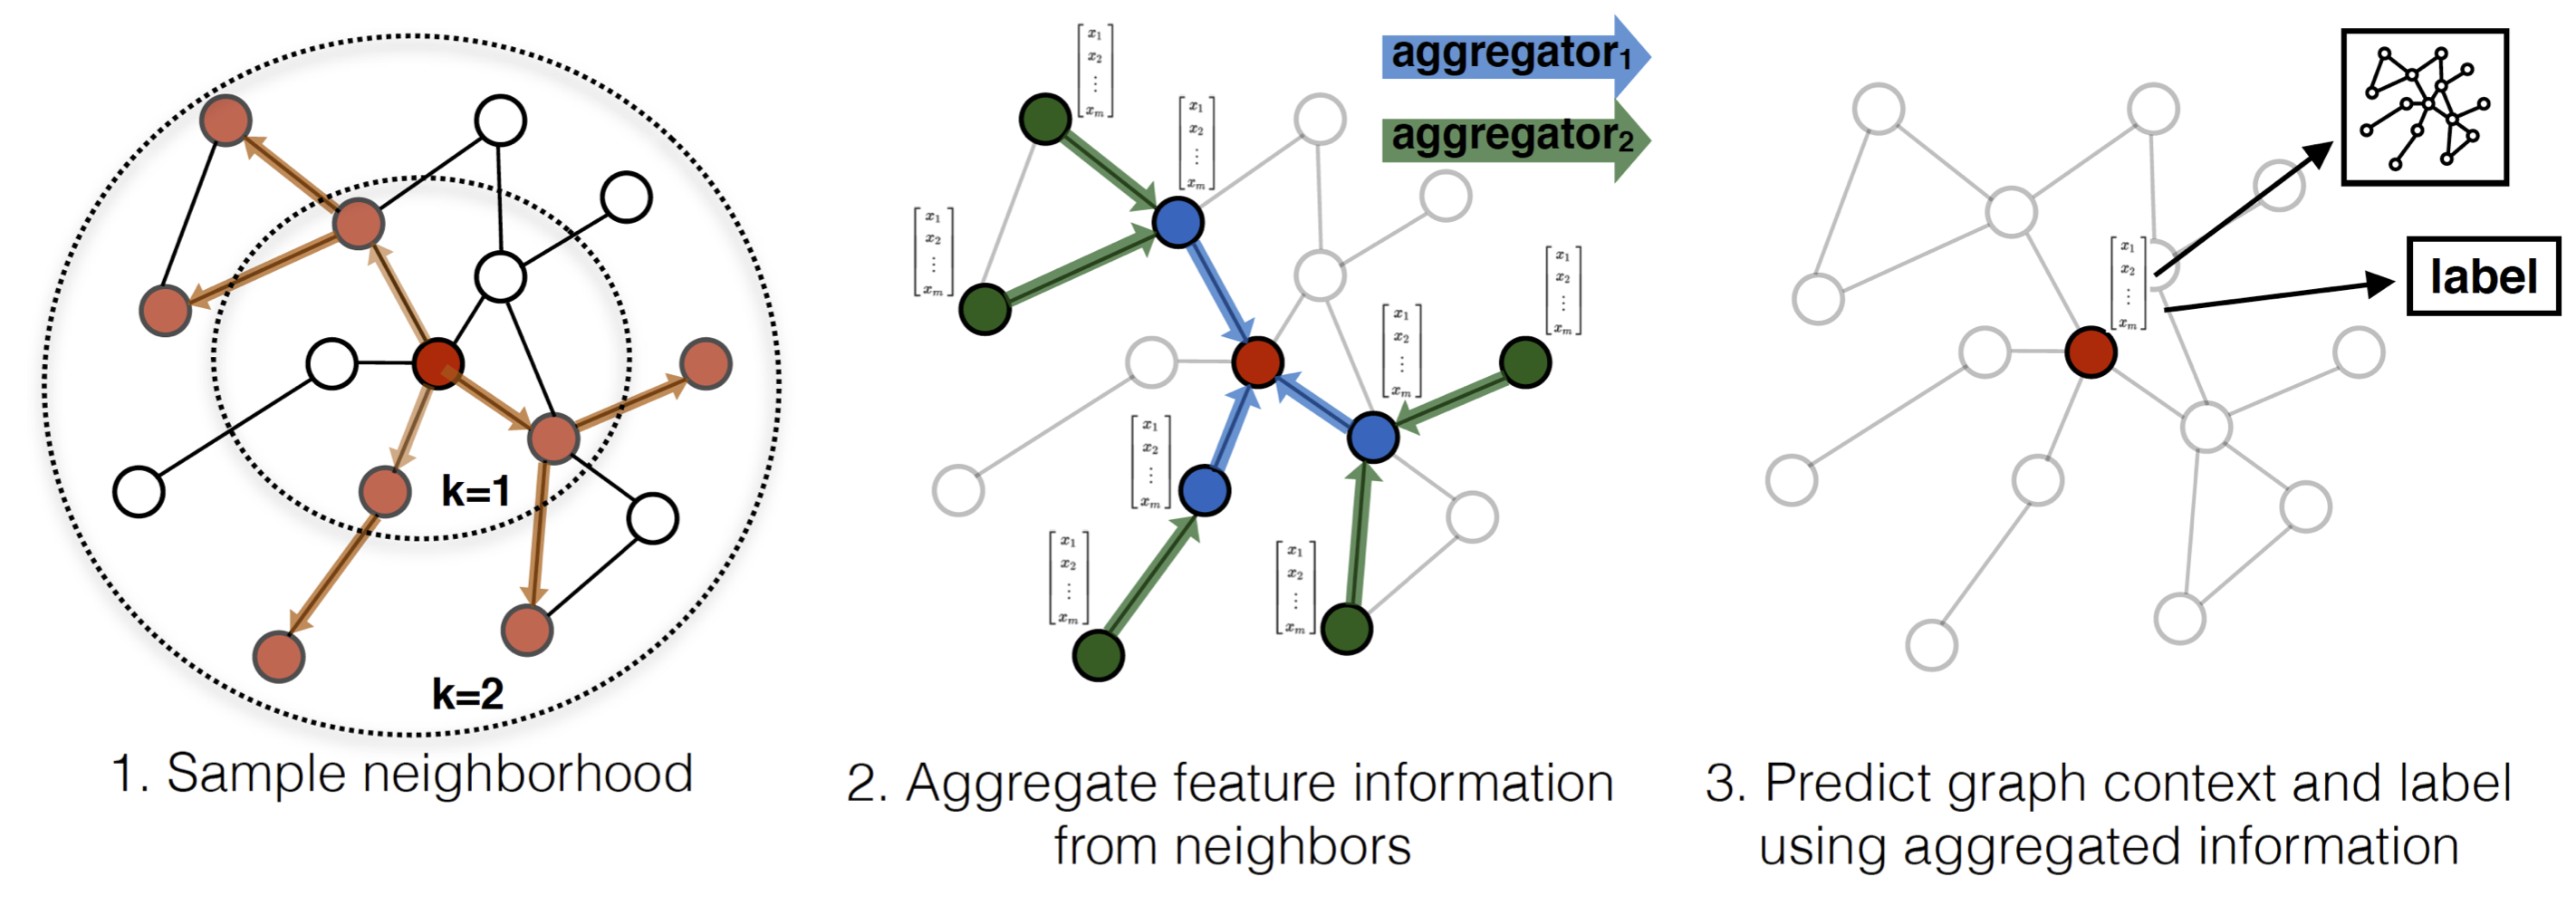
\includegraphics[width=0.99\textwidth]{sample_and_agg.png}
\caption{Visual illustration of the \name\ sample and aggregate approach.}
\vspace{-15pt}
\label{fig:overview}
\end{figure}


We evaluate our algorithm on three node-classification benchmarks, which test \name's ability to generate useful embeddings on unseen data. 
We use two evolving document graphs based on citation data and Reddit post data (predicting paper and post categories, respectively), and a multi-graph generalization experiment based on a dataset of protein-protein interactions (predicting protein functions). 
  Using these benchmarks, we show that our approach is able to effectively generate representations for unseen nodes and outperform relevant baselines by a significant margin: across domains, our supervised approach improves classification F1-scores by an average of 51\% compared to using node features alone and \name\ consistently outperforms a strong, transductive baseline \cite{perozzi2014deepwalk}, despite this baseline taking ${\sim}100\times$ longer to run on unseen nodes.
We also show that the new aggregator architectures we propose provide significant gains (7.4\% on average) compared to an aggregator inspired by graph convolutional networks \cite{kipf2016semi}.
 Lastly, we probe the expressive capability of our approach and show, through theoretical analysis, that \name\ is capable of learning structural information about a node's role in a graph, despite the fact that it is inherently based on features (Section \ref{sec:theory}). 